\documentclass{article}
\usepackage[margin = 0.15in,landscape]{geometry}
\usepackage{multicol}
\usepackage{array}
\usepackage{amsmath}
\usepackage{amssymb}
\usepackage{lmodern}
\usepackage{graphicx}
\usepackage{enumitem}
\usepackage{wasysym}
\setlength\parindent{0pt}
\renewcommand{\baselinestretch}{0.75}


\begin{document}
\begin{multicols*}{3}
    Marissa Palamara\par 
    ASEN 3200\par 
    Fall 2020
    \vspace{-0.5cm}
    \setlist{nolistsep}

    % ----- The Two-Body Problem ----- %
    \subsection*{Two-Body Problem}
    Newton's Law: $\Sigma \vec{F}=\frac{d(m\vec{v})}{dt}=m\vec{a}$ \par
    Universal Law of Gravitation: $\vec{F}_g=-\frac{Gm_1m_2}{r^2}\frac{\vec{r}}{|\vec{r}|}$\par 
    Apply Newton's Laws to a two-body problem with the assumptions:
    \begin{enumerate}
        \itemsep0em
        \item Only system force: Gravity $\rightarrow$ acts along the line joining the centers of the bodies.
        \item Mass of each body is constant.
        \item Treat each body as a spherically symmetrical point mass with uniform density.
    \end{enumerate}
    \subsection*{Orbits}
    \textbf{Elliptical Orbits}:\par
    \textbf{Orbital Properties:}
    \begin{itemize}
        \itemsep0em
        \item a = semimajor axis
        \item b = semiminor axis
        \item p = semiperimeter
        \item $r_a/r_p$ = radii of apoapsis/periapsis
        \item $\vec{e}$ = eccentricity
    \end{itemize}
    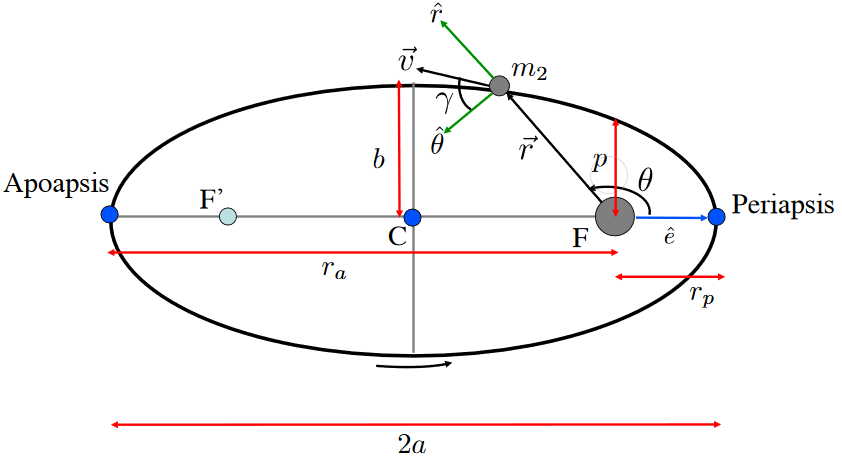
\includegraphics[width=\linewidth]{Figures/orbital_properties.png}

    \textbf{Useful Equations:}\par
    $a = \frac{1}{2}(r_a+r_p)$\par 
    $p=\frac{b^2}{a}=a(1-e^2)=\frac{h^2}{\mu}$\par 
    $r_a = \frac{p}{1-e}=a(1+e)$\par 
    $r_p = \frac{p}{1+e}=a(1-e)$\par
    $e = \frac{r_a-r_p}{r_a+r_p}$ = $\frac{c}{a}$ = $\frac{\sqrt{a^2-b^2}}{a}$ = $\sqrt{1+\frac{2h^2\varepsilon}{\mu^2}}$\par 
    $b = a\sqrt{1-e^2}$ \par
    Angular Momentum: $\vec{h} = \vec{r} \times \vec{v}$ = $\sqrt{\mu a (1-e^2)}$ \par
    Eccentricity Vector: $\vec{e} = \frac{\vec{v} \times \vec{h}}{\mu}-\frac{\vec{r}}{r}$\par
    Specific Energy: $\varepsilon = \frac{v^2}{2}-\frac{\mu}{r}$ = $\frac{\mu^2(e^2-1)}{2h^2}$\par
    \begin{itemize}
        \itemsep0em
        \item $\varepsilon < 0$ Motion of Body 2 is bounded wrt Body 1
        \item $\varepsilon \ge 0$ Motion of Body 2 is unbounded wrt Body 1
    \end{itemize}
    Conic Equation: $r = \frac{h^2/\mu}{1+e\cos{\theta}}$ = $\frac{p}{1+e\cos{\theta}}$\par 
    Vis-Viva Equation: $v=\sqrt{\frac{2\mu}{r}-\frac{\mu}{a}}$\par
    %\vspace{1.5cm}
    \textbf{True Anomaly:} 
    \begin{itemize}
        \itemsep0em
        \item $\theta$ or $\nu$
        \item Measured from periapsis, $\vec{e}$ to radius, $\vec{r}$
        \item $\theta = 0$ at periapsis
        \item $0^\circ > \theta > 180^\circ \rightarrow m_2$ moving away from periapsis
        \item $180^\circ < \theta < 360^\circ m_2$ moving toward periapsis
    \end{itemize}
    \textbf{Flight Path Angle:} 
    \begin{itemize}
        \itemsep0em
        \item $\tan{\gamma} = \frac{e\sin{\theta}}{1+e\cos{\theta}} = \frac{v_r}{v_{\theta}}$
        \item $v_r = \frac{\mu}{h}e\sin{\theta}$ and $v_\theta = \frac{\mu}{h}(1+e\cos{\theta})$
        \item $\gamma > 0$ when $v_r>0$ and $\theta>0\rightarrow$ $m_2$ moving away from periapsis
    \end{itemize}
     
    \textbf{Perifocal Frame:}  
    \begin{itemize}
        \itemsep0em
        \item $\hat{p}$, $\hat{q}$, $\hat{w}$
        \item $\vec{r} = r\hat{r} = r\cos{\theta}\hat{p} + r\sin{\theta}\hat{q}$
        \item $\vec{v} = \frac{\mu}{h}[-\sin{\theta}\hat{p}+(e+\cos{\theta})\hat{q}]$
    \end{itemize}
    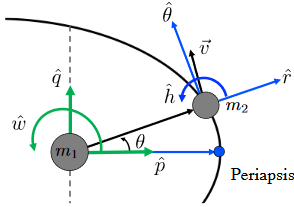
\includegraphics[width=0.5\linewidth]{Figures/perifocal_plane.png}
    
    \textbf{Kepler's Law:} A line joining a planet and the Sun sweep out equal areas during equal intervals of time.\par 
    \textbf{Elliptical Orbits:} $\mathbb{P}=2\pi\sqrt{\frac{a^3}{\mu}}$, $\varepsilon<0$\par
    \textbf{Mean Motion:} $n=\sqrt{\frac{\mu}{a^3}}$ - mean angular rate of motion\par 
    \textbf{Circular Orbits:}
    \begin{itemize}
        \itemsep0em
        \item $r = a$, $\vec{v} \perp \vec{r}$, and $\gamma = 0$ everywhere
        \item $v_c=\sqrt{\frac{\mu}{r}}$
    \end{itemize}
    \textbf{Parabolic Orbits:}
    \begin{itemize}
        \itemsep0em
        \item $e=1$, $a=\inf$, $r_a=$ undefined
        \item Conic equation applies still
        \item $p = \frac{h^2}{\mu}$
        \item $\varepsilon=0$ everywhere
        \item $v = \sqrt{\frac{2\mu}{r}}=v_{esc}$
    \end{itemize}
    \textbf{Hyperbolic Orbits:}
    \begin{itemize}
        \itemsep0em
        \item $v>v_{esc}$, $e>1$, $\varepsilon>0$, $a<0$
        \item $r_p=|a|(e-1)$
        \item $p=|a|(e^2-1)=a(1-e^2)$
        \item $r=\frac{a(1-e^2)}{1+e\cos{\theta}}=\frac{|a|(e^2-1)}{1+e\cos{\theta}}$
        \item at $r = \infty$, $\varepsilon = \frac{-\mu}{2a}=\frac{v^2_{\infty}}{2}\rightarrow v_{\infty}=\sqrt{\frac{\mu}{|a|}}$
        \item $\theta_{\infty} = \pm\cos^{-1}\left({\frac{-1}{e}}\right)$
        \item $v^2=v^2_{esc}+v^2_{\infty}$
        \item turning angle: $\frac{\delta}{2}+90^\circ=\theta_\infty$, $\delta = 2\sin^{-1}({\frac{1}{e}})$
    \end{itemize}
    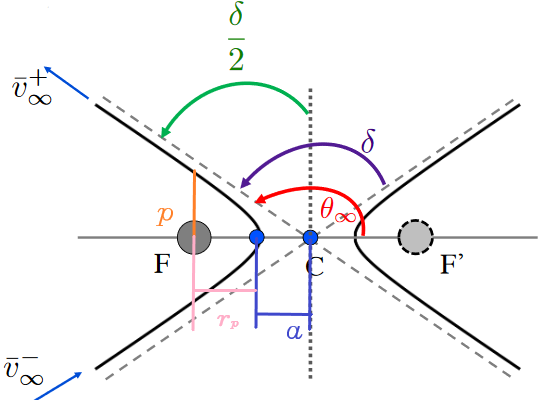
\includegraphics[width=0.5\linewidth]{Figures/hyperbolic_orbit.png}

    % ----- The Anomalies ----- %
    \subsection*{The Anomalies}
    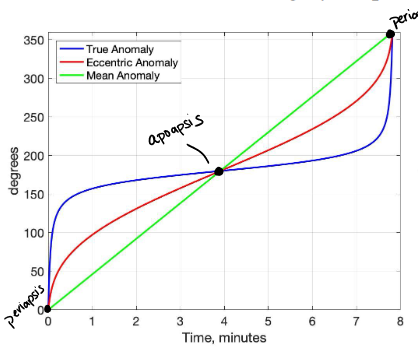
\includegraphics[width=\linewidth]{Figures/The_Anomalies.png}
    \begin{itemize}
        \item True anomaly
        \begin{itemize}
            \item Advances quickly from periapsis
            \item Advances slowly from apoapsis
        \end{itemize}
        \item Mean anomaly, $M$
        \begin{itemize}
            \item Computed from time and mean motion
            \item $M = n(t-t_p)$
            \item Advances at constant rate in elliptical orbit
        \end{itemize}
        \item Eccentric anomaly, $E$
        \begin{itemize}
            \item Angle that helps translate from true anomaly to mean anomaly
            \item Advances at rate between True and Mean anomaly 
        \end{itemize}
    \end{itemize}

    \textbf{Kepler's Equation:} $M=n(t-t_p)=E-e\sin{E}$\par 
    Everything in rads!

    Finding E:\par 
    \begin{itemize}
        \item Choose an initial estimate of E:
        \begin{itemize}
            \item $M_e < \pi \rightarrow E = M_e + e/2 \quad M_e > \pi \rightarrow M_e - e/2$
        \end{itemize}
        \item $f(E) = E-e\sin{E}-M_e$
        \item $f'(E) = 1-e\cos{E}$
        \item Iterate and update $E_i$\par 
        $E_{i+1} = E_i - \frac{f(E_i)}{f'(E_i)}$ 
    \end{itemize}

    Switching between the Anomalies:\par
    \begin{itemize}
        \item $\cos{E} = \frac{e+\cos{\theta}}{1+e\cos{\theta}}$
        \item $\tan{\frac{E}{2}}=\sqrt{\frac{1-e}{1+e}}\tan{\frac{\theta}{2}}$
        \item $\tan{\frac{\theta}{2}}=\sqrt{\frac{1-e}{1+e}}\tan{\frac{E}{2}}$
        \item $r = a(1-e\cos{E})=\frac{p}{1+e\cos{\theta}}=\frac{a(1-e^2)}{1+e\cos{\theta}}$
        \item $\sin{\theta}=\frac{b}{r}\sin{E}$
    \end{itemize}

    To find time between A and B, with $a$,$e$,and $\theta$ of A and B known,\par 
    $t_B-t_A=(t_B-t_p)-(t_A-t_p)$
    \newpage
    \textbf{Hyperbolic Anomaly, H}\par 
    Use an equilateral hyperbola to determine H: $e = \sqrt{2}$\par 
    \begin{itemize}
        \item $M_h=\sqrt{\frac{\mu}{|a|^3}}(t-t_p)=e\sinh{H}-H$
        \item $\tanh{\frac{H}{2}}=\sqrt{\frac{e-1}{e+1}}\tan{\frac{\theta^*}{2}}$
        \item $\tanh{\frac{\theta^*}{2}}=\sqrt{\frac{e-1}{e+1}}\tan{\frac{H}{2}}$
    \end{itemize}

    \textbf{Parabolic Orbits}\par 
    Barkers Equation: 
        \begin{equation*}
            \begin{array}{l}
                \bullet \sqrt{\frac{\mu}{p^3}}(t-t_p)=\frac{\mu^2}{h^2}(t-t_p)=M_p=\frac{1}{6}\tan^3{\frac{\theta}{2}}+\frac{1}{2}\tan{\frac{\theta}{2}}\\
                \bullet \tan{\frac{\theta}{2}}=\left(3M_p+\sqrt{(3M_p)^2+1}\right)^{1/3}\\
                -\left(3M_p+\sqrt{(3M_p)^2+1}\right)^{-1/3}
            \end{array}
        \end{equation*}
    
    % ----- 3D Orbits ----- %
    \subsection*{3D Orbits}
    How many variables required to completely describe the state of a satellite?\par 
    6: 3 position and 3 velocity\par 
    OR\par 
    Can also describe a satellite's states by set of orbital elements:
    \begin{itemize}
        \item Size and shape: $a,e$
        \item Orientation of the orbit plane: $i,\Omega$
        \item Orientation of the orbit within the orbit plane: $\omega$
        \item Location of the satellite on the orbit: $\theta$ $(M,E,t-t_p)$
    \end{itemize}

    \textbf{Inclination, $i$:}\par 
    \begin{itemize}
        \item Angular tile of the orbital plane relative to $\hat{X}\hat{Y}$ and measured 
        between orbit normal, $\hat{h}$ and $\hat{Z}$
        \item Equatorial Orbit: $i=0^\circ, 180^\circ$
        \item Polar Orbit: $i=90^\circ$
        \item Prograde Orbit: $i=[0^\circ,90^\circ]$
        \item Retrograde Orbit: $i=[90^\circ,180^\circ]$
        \item $\cos{i}=\frac{\hat{Z}\cdot\vec{h}}{|\hat{Z}||\vec{h}|}\rightarrow\cos{i}=\frac{h_z}{h}$
    \end{itemize}

    \textbf{Right Ascension of the Ascending Node, $\Omega$:}
    \begin{itemize}
        \item Angle from the reference direction, $\hat{X}$, to the ascending node.
        \item Line of Nodes: $\vec{n}=\hat{Z}\times\vec{h}$
        \item $\cos{\Omega}=\frac{\hat{X}\cdot\vec{n}}{|\hat{X}||\vec{n}}=\frac{n_x}{n}$
        \item Quadrant Check:
            \begin{itemize}
                \item $\vec{n}\cdot\hat{Y}>0\rightarrow 0 < \Omega < 180^\circ$
                \item $\vec{n}\cdot\hat{Y}<0\rightarrow 180^\circ < \Omega < 360^\circ$
                \item Between $0-2\pi$
            \end{itemize}
    \end{itemize}

    \textbf{Argument of Periapsis, $\omega$ (AOP):}
    \begin{itemize}
        \item Measured between the lines of nodes $\vec{n}$ and the eccentricity vector, $\vec{e}$
        \item Locates the closest point of the orbit
        \item Measured within the plane, varies from $0-2\pi$
        \item $\cos{\omega}=\frac{\vec{n}\cdot\vec{e}}{|\vec{n}||\vec{e}|}$
        \item Quadrant Check:
            \begin{itemize}
                \item $\vec{e}\cdot\hat{z}>0\rightarrow 0<\omega<180^\circ$
                \item $\vec{e}\cdot\hat{z}<0\rightarrow 180^\circ<\omega<360^\circ$
            \end{itemize}
    \end{itemize}
    \vspace{1cm}
    \textbf{True Anomaly, $\theta$:}
    \begin{itemize}
        \item Location of the spacecraft within the orbit
        \item Varies from $0-2\pi$
        \item $\vec{r}\cdot\vec{e}=|\vec{r}||\vec{e}|\cos{\theta}$
        \item $\cos{\theta}=\frac{\vec{r}\cdot\vec{e}}{|\vec{r}||\vec{e}|}$
        \item Quadrant Check:
            \begin{itemize}
                \item $\vec{r}\cdot\vec{v}>0\rightarrow 0 < \theta < 180^\circ$
                \item $\vec{r}\cdot\vec{v}<0\rightarrow 180^\circ<\theta<360^\circ$
            \end{itemize}
    \end{itemize}

    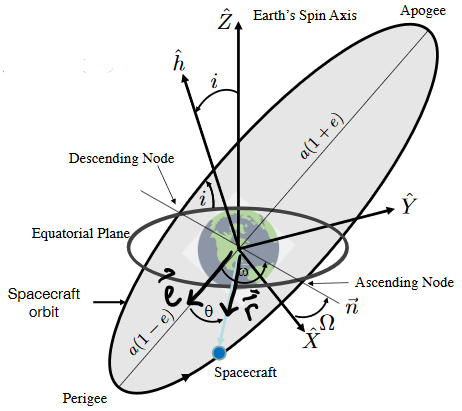
\includegraphics[width=\linewidth]{Figures/Orbital_Elements.png}

    \textbf{Converting Position and Velocity to Orbital Elements:}\par
    \begin{itemize}
        \item Given $X = [\vec{r},\vec{v}]$
        \item Compute vectors and their magnitudes:
        \begin{equation*}
            \begin{array}{lll}
                \vec{h}=\vec{r} \times \vec{v} & \vec{n} = \hat{Z} \times \vec{h} & \vec{e}=\frac{\vec{v} \times \vec{h}}{\mu}-\frac{\vec{r}}{r}\\
                h=|\vec{h}| & n=|\vec{n}| & e=|\vec{e}|
            \end{array}
        \end{equation*}
        \item Compute energy to get $a$:
        \begin{equation*}
            \begin{array}{ll}
                \varepsilon=\frac{v^2}{2}-\frac{\mu}{r} & a=-\frac{\mu}{2\varepsilon}\\
                p=\frac{h^2}{\mu} & a = \frac{p}{1-e^2}
            \end{array}
        \end{equation*}
        \item Compute inclination \& Orientation Angles from above
            \begin{itemize}
                \item $\Omega\rightarrow \text{If} (n_y<0), \Omega=360^\circ-\Omega$
                \item $\omega\rightarrow \text{If} (e_z<0), \omega=360^\circ-\omega$
                \item $\theta\rightarrow \text{If} (\vec{r}\cdot\vec{v}<0), \theta=360^\circ-\theta$
            \end{itemize}
    \end{itemize}

    \textbf{What about...?}
    \begin{itemize}
        \item What is $\Omega$ for an elliptical equatorial orbit?
            \begin{itemize}
                \item Undefined, used true longitude of periapse: $\tilde{\omega}_{true}$
                \item $\cos{\tilde{\omega}_{true}}=\frac{\hat{X}\cdot\vec{e}}{|\hat{X}||\vec{e}|}$ where $\hat{X}=[1,0,0]$
                \item If $e_y<0\rightarrow \tilde{\omega}_{true}=360^\circ-\tilde{\omega}_{true}$
            \end{itemize}
        \item What is $\omega$ for a circular orbit? (No perigee) $\rightarrow$ undefined!
        \item Use arugment of latitude
            \begin{itemize}
                \item $\cos{u}=\frac{\vec{n}\cdot\vec{r}}{|\vec{n}||\vec{r}|}\rightarrow \text{If } (r_z<0), \text{then } u = 360^\circ -u$
            \end{itemize}
        \item Circular, equatorial orbits? Both $\omega$ and $\Omega$ undefined!
            \begin{itemize}
                \item $\cos{\lambda_{true}}=\frac{\hat{X}\cdot{\vec{r}}}{|\hat{X}||\vec{r}|}\rightarrow \text{If } (r_y<0), \text{then } \lambda_{true}=360^\circ - \lambda_{true}$
            \end{itemize}
    \end{itemize}

    % ----- Coordinate Frames ----- %
    \subsection*{Coordinate Frames}
    \textbf{Ecliptic Plane:}\par 
    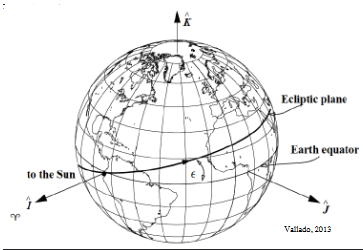
\includegraphics[width=0.5\linewidth]{Figures/ecliptic_plane.png}
    \begin{itemize}
        \item Mean plane of the Earth's orbit around the Sun.
        \item Earth's equatorial plane is inclined about 23.5$^\circ$ relative to ecliptic.
        \item Vernal Equinox $\vernal$: 
            \begin{itemize}
                \item intersection of Sun's path relative to the Earth with the equatorial plane, as Sun moves from South to North.
                \item Occurs at ascending node of the Sun as viewed from Earth
                \item Used as reference direction for defining intertial reference frames
            \end{itemize}
    \end{itemize}

    \textbf{ICRF: International Celestial Reference Frame}\par 
    \begin{itemize}
        \item Close representation of intertial frame (rotates a little)
        \item Nonrotating with respect to extragalactic radio sources (quasars)
        \item Center: Barycenter of the Solar System
    \end{itemize}

    \textbf{Earth-Centered Mean Equatorial J2000 System (EME2000):}
    \begin{itemize}
        \item Origin: Earth Center
        \item $\hat{X}$: Vernal Equinox at 1/1/2000 12:00:00 TT
        \item $\hat{Z}$: Normal to the mean equatorial plane of Earth at the J2000 epoch (Spin axis of Earth)
        \item $\hat{Y}$: Completes right hand coordinate frame
    \end{itemize}

    \textbf{Earth-Centered Mean Orbit and Equinox of J2000 (EMO2000):}
    \begin{itemize}
        \item Origin: Earth Center
        \item $\hat{X}$: Vernal Equinox at 1/1/2000 12:00:00 TT
        \item $\hat{Z}$: Orbit normal vector at same time
        \item $\hat{Y}$: Completes right hand coordinate frame
        \item Differs from EME2000 by ~23.4393$^\circ$
    \end{itemize}
    \newpage
    \textbf{Earth-Centered Earth-Fixed:}\par 
    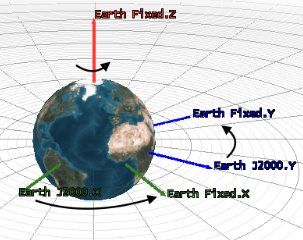
\includegraphics[width=0.5\linewidth]{Figures/Earth_fixed.png}[H]
    \begin{itemize}
        \item Origin: Earth Center
        \item $\hat{X}$: Osculating vector from center of Earth toward the equator along the Prime Meridian (rotates with Earth)
        \item $\hat{Z}$: Aligned with Earth's spin axis
        \item $\hat{Y}$: Completes right hand coordinate frame
    \end{itemize}

    \textbf{Topocentric Horizon System:}\par 
    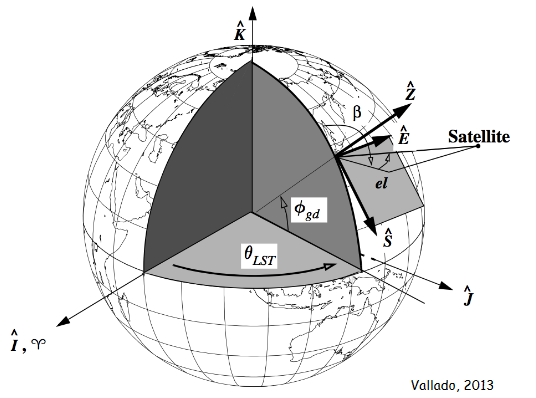
\includegraphics[width=0.5\linewidth]{Figures/SEZ.png}
    \begin{itemize}
        \item Usefule for observing satellites and sensor systems
        \item Origin = site on Earth
        \item SEZ frame rotates with site
        \item Local Horizon forms fundamental plane:
            \begin{itemize}
                \item $\hat{S}$: Points due South
                \item $\hat{E}$: Points due East
                \item $\hat{Z}$: Points radially outward
                \item $\beta$: Azimuth, angle measured from North, clockwise to location beneath object of interest
                \item el: Elevation, measured from local horizon, positive up to the object $[-90^\circ,90^\circ]$
            \end{itemize}
    \end{itemize}

    \textbf{Perifocal Coordinate System:}\par 
    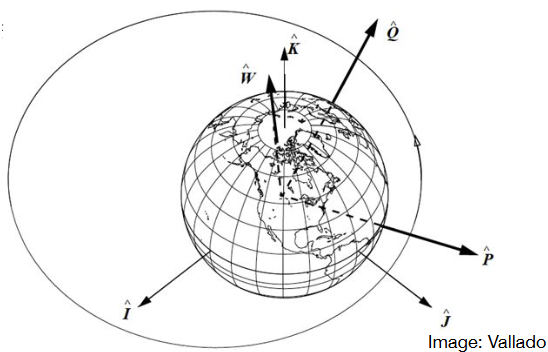
\includegraphics[width=0.5\linewidth]{Figures/perifocal_orbit.png}
    \begin{itemize}
        \item Fundamental Plane: Satellite Orbit
        \item Origin: Center of Earth
        \item $\hat{P}$: Points toward perigee
        \item $\hat{Q}$: $90^\circ$ from $\hat{P}$ axis in direction of satellite motion
        \item $\hat{W}$: normal to the orbit 
    \end{itemize}

    \subsection*{Coordinate Frame Transformations}
    \textbf{Generic:}
    \begin{equation*}
        \begin{array}{lll}
            X,I & R_1(\alpha) & ROT1(\alpha) = 
            \begin{bmatrix}
                1 & 0 & 0\\
                0 & c\alpha & s\alpha\\
                0 & -s\alpha & c\alpha
            \end{bmatrix}\\
            Y,J & R_2(\alpha) & ROT2(\alpha) = 
            \begin{bmatrix}
                c\alpha & 0 & -s\alpha\\
                0 & 1 & 0\\
                s\alpha & 0 & c\alpha
            \end{bmatrix}\\
            Z,K & R_3(\alpha) & ROT3(\alpha) = 
            \begin{bmatrix}
                c\alpha & s\alpha & 0\\
                -s\alpha & c\alpha & 0\\
                0 & 0 & 1
            \end{bmatrix}
        \end{array}
    \end{equation*}

    \textbf{Perifocal-Rotating Transformation:}\par 
    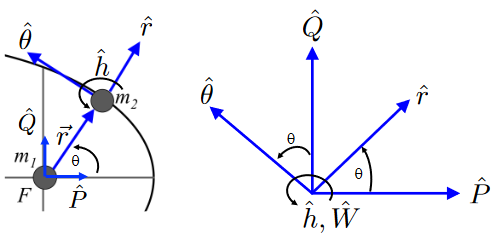
\includegraphics[width=\linewidth]{Figures/peri-rot.png}
    \begin{equation*}
        \begin{bmatrix}
            r\\
            \theta\\
            h
        \end{bmatrix}
        =
        \begin{bmatrix}
            c\theta & s\theta & 0\\
            -s\theta & c\theta & 0\\
            0 & 0 & 1
        \end{bmatrix}
        \begin{bmatrix}
            P\\
            Q\\
            W
        \end{bmatrix}
    \end{equation*}

    \textbf{Express position and velocity in PQW frame to Cartesian:}\par 
    $\vec{r}_{PQW} = r\cos{\theta}\hat{P}+r\sin{\theta}\hat{Q}=
    \begin{bmatrix}
        \frac{p\cos{\theta}}{1+e\cos{\theta}}\\
        \frac{p\sin{\theta}}{1+e\cos{\theta}}\\
        0
    \end{bmatrix}
    $\par
    $\vec{v}_{PQW} =
    \begin{bmatrix}
        \dot{r}\cos{\theta}-r\dot{\theta}\sin{\theta}\\
        \dot{r}\sin{\theta}+r\dot{\theta}\cos{\theta}\\
        0
    \end{bmatrix}
    =
    \begin{bmatrix}
        -\sqrt{\frac{\mu}{p}}\sin{\theta}\\
        \sqrt{\frac{\mu}{p}}(e+\cos{\theta})\\
        0
    \end{bmatrix}
    $\par 
    $[C]=R_3(-\Omega)R_1(-i)R_3(-\omega)$\par 
    $\vec{r}_{xyz} = [C]\vec{r}_{PQW} \quad \vec{v}_{xyz}=[C]\vec{v}_{PQW}$\par 
    \textbf{To go from XYZ to PQW:}\par 
    $\vec{r}_{PQW}=R_3(\omega)R_1(i)R_3(\Omega)\vec{r}_{xyz}$

    \subsection*{Ground Track}
    Earth rotates 15.04$^\circ$/hour eastward beneath the satellite.\par 
    Ground track advances westward at this rate.\par 
    We can relate the distance between successive ground track crossing to the
    orbital period using Earth's rotation:\par 
    $\mathbb{P}=\frac{D}{15.04^\circ/hour}$

\end{multicols*}  
\end{document}
